\documentclass[11pt]{article}
\usepackage{amsmath}
\usepackage{geometry}                % See geometry.pdf to learn the layout options. There are lots.
\geometry{letterpaper}                   % ... or a4paper or a5paper or ... 
%\geometry{landscape}                % Activate for for rotated page geometry
%\usepackage[parfill]{parskip}    % Activate to begin paragraphs with an empty line rather than an indent
\usepackage{graphicx}
\usepackage{amssymb}
\usepackage{epstopdf}
\DeclareGraphicsRule{.tif}{png}{.png}{`convert #1 `dirname #1`/`basename #1 .tif`.png}

\title{Archipelago}
\author{Jeet Sukumaran}
%\date{}                                           % Activate to display a given date or no date

\begin{document}
\maketitle
\section*{Introduction}
Archipelago is a forward-time simulation of macro-evolutionary diversification processes in a spatially-explicit framework.
The motivation for this simulator is to provide for null distributions of diversity, i.e., numbers of species or lineages found in different regions, under the model being simulated.

\section*{The Simulation Model}

\subsection*{The Diversification Process}
The birth-death process has two parameters.
The birth rate, $\lambda$, is the probability that each species in the system speciates, or splits into two daughter species.
The death rate, $\mu$, is the probability that each species in the system goes extincts.
A special case of the birth-death process is when the death rate, $\mu$, is 0, in which case we have a pure-birth process, which is also referred to as the \textit{Yule} model.

In the pure birth process, the expected number of lineages, $E(n)$ at time $t$ is given by:
\begin{align*}
E(n) = e^{\lambda t},
\end{align*}
corresponding to population growth equations of the same form.

With extinction, the expected number of lineages, $E(n)$ at time $t$ is:
\begin{align*}
E(n) = e^{(\lambda-\mu) t}.
\end{align*}

\subsection*{The Geographic Template}

The spatial aspect of the simulation model is represented by the \textit{geographical template}, which the defines the fundamental atomic spatial units of the simulation, \textit{regions}, and the connectivity between these units, which determines the rate of dispersal of lineages from one region to another.

The geographical template is specified as a $M \times M$ matrix, where $M$ is the number of regions in the system and the value of cell $M_{i,j}$ specifies the probability of dispersal from the $i^{th}$ region to the $j^{th}$ region.
The rows of the matrix are required to sum to 1, and cell $M_{i,i}$ represents the probability of no dispersal.

For example, the following schematic representation of the geographical template:

\begin{center}
	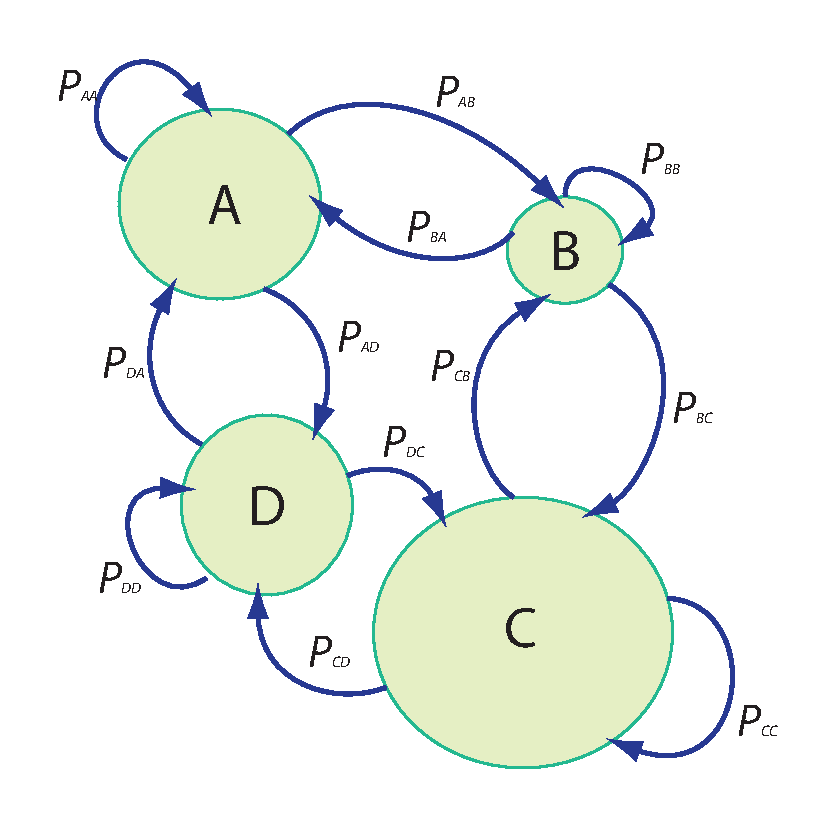
\includegraphics[scale=0.3]{generic-geographical-template.pdf}
\end{center}

would be represented by the following matrix:

\begin{center}
    \begin{tabular}{c|cccc}
          & A & B & C & D\\
		\hline	             
        A & $P_{AA}$ & $P_{AB}$ & $P_{AC}$ & $P_{AD}$ \\
        B & $P_{BA}$ & $P_{BB}$ & $P_{BC}$ & $P_{BD}$ \\
        C & $P_{CA}$ & $P_{CB}$ & $P_{CC}$ & $P_{CD}$ \\
        D & $P_{DA}$ & $P_{DB}$ & $P_{DC}$ & $P_{DD}$ \\
    \end{tabular}
\end{center}		        

\subsection*{Speciation Modes}

Two types of speciation modes are supported: \textit{sympatric} and \textit{allopatric} speciation.
In sympatric speciation, a speciation event results in one region receiving both daughter lineages while the remaining regions receive just one of the two (the same one for all the remaining regions):

\begin{center}
	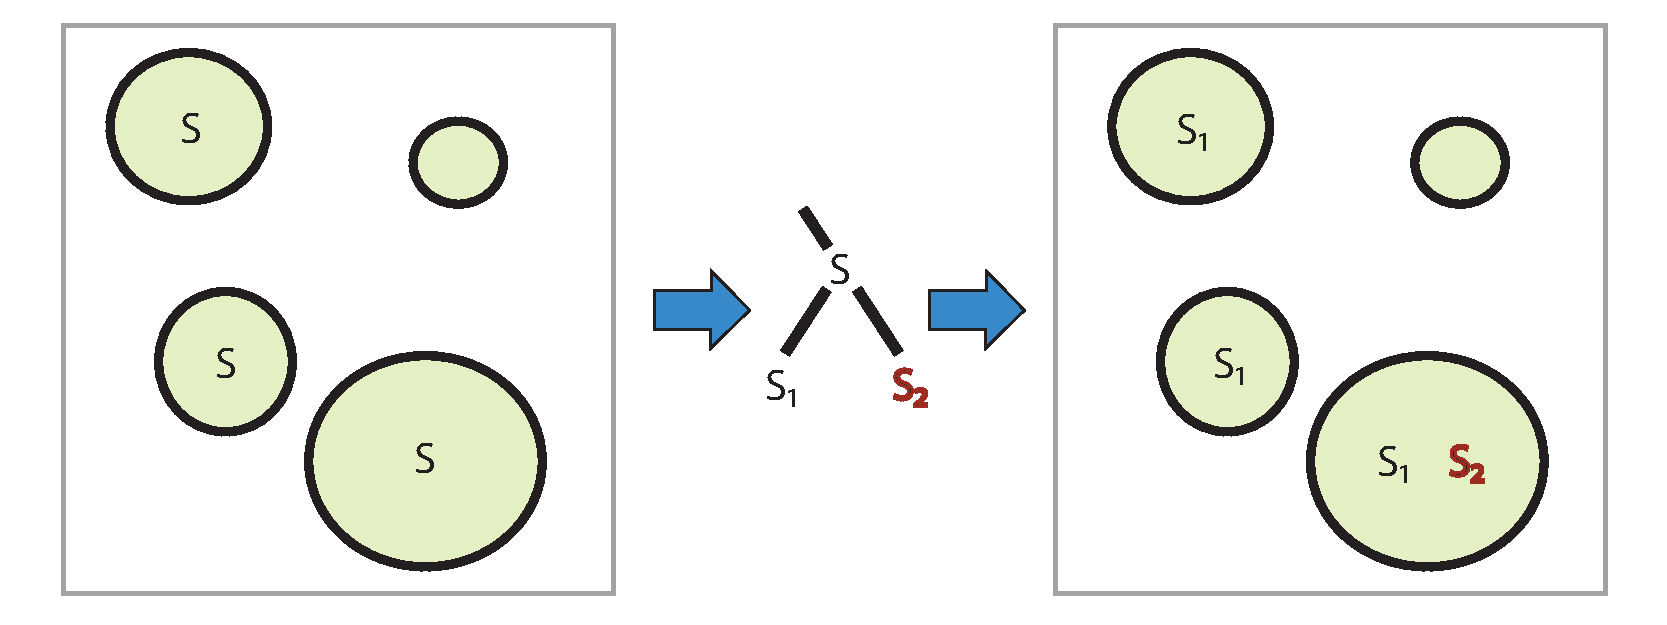
\includegraphics[scale=0.3]{sympatric-speciation.pdf}
\end{center}


In allopatric speciation, one region region receives one of the daughters, while all the others receive the other:

\begin{center}
	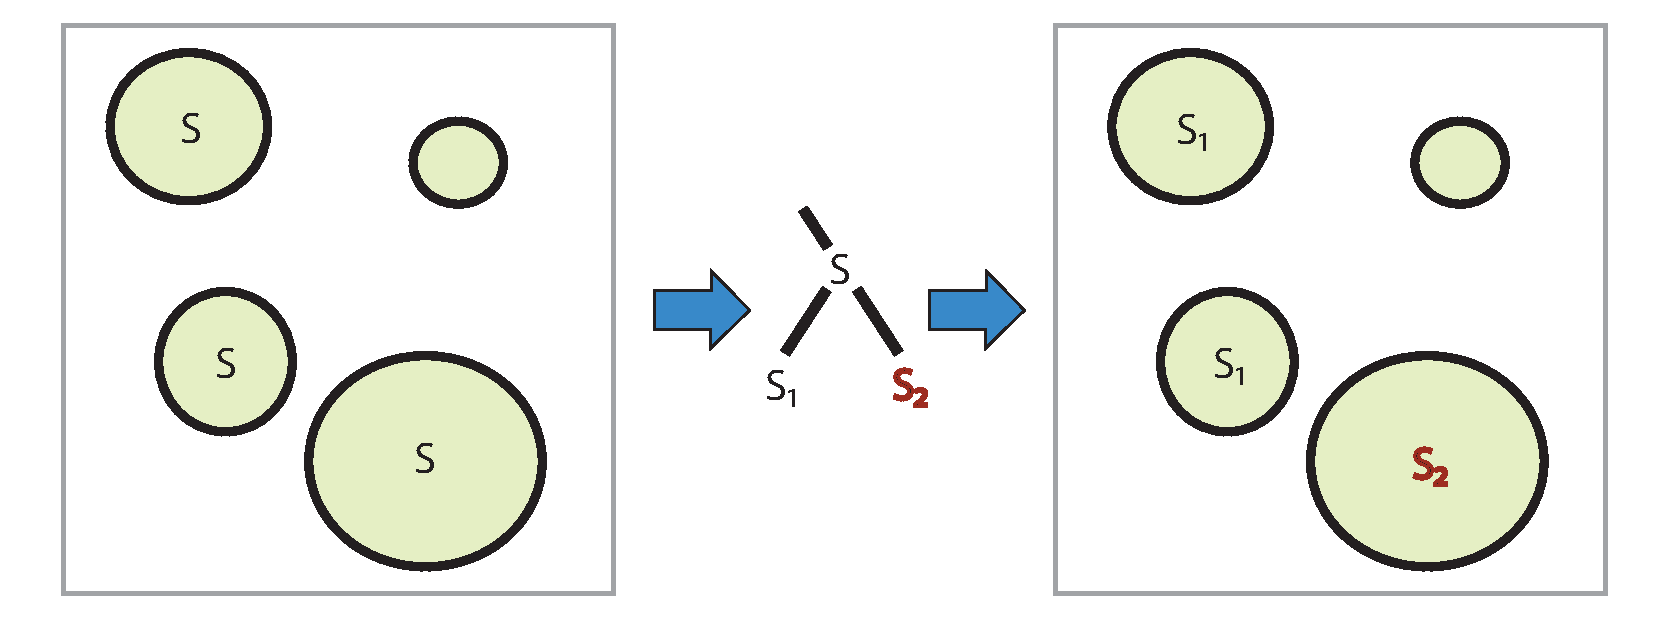
\includegraphics[scale=0.3]{allopatric-speciation.pdf}
\end{center}

\subsection*{The Simulation Procedure}
The simulation is set up by specifying the birth rate, $\lambda$, the death rate, $\mu$, and the geographical template as a matrix of dispersal probabilities, as well as a random seed to use.
The birth rate, death rate and random seed are specified as command line arguments to the program, while the dispersal probability matrix is given a text file provided to the program.

The termination condition for the simulation also needs to be specified.
Two types of termination conditions are supported.
The first, \textit{target diversity}, specifies the number of species or lineages that need to be generated.
The second, \textit{generation limit}, specifies the number of generations that need to be run, irrespective of the number of species or lineages that are generated.
The ``target diversity'' termination condition is ideally suited for generating distributions of diversity that match some observed total diversity, to statistically compare the distributions of the same total diversity under random diversification and dispersal against that observed, to see whether additional factors might be operating in the observed system.

Once the simulation is set up with the appropriate parameters and termination condition, a particular region is \textit{seeded} with an initial species or lineage. 
The main simulation cycle then runs until the specified termination condition is reached.

The main simulation cycle consists of two phases: the \textit{dispersal} phase and the \textit{diversification} phase.

In the dispersal phase, for each species or lineage in each region, a dispersal destination is selected based on the dispersal probabilities defined in the geographical template.
This destination may the same as the source region, or it may be another region in the system.
If the destination region is the same as the source region, or if the species or lineage already exists in the destination region, then no colonization of a new region occurs.
Otherwise, the destination region is added to the range of the species.

In the diversification phase, a uniform random number, $u \sim U(0,1)$ is generated.
If $u < \lambda$ then a speciation event is modeled, while if $\lambda < u < \lambda + \mu$ then an extinction event is modeled.
A speciation event is modeled by splitting the speciating lineage into two daughter species.
Each daughter species inherits the range of their parent (i.e., the speciating lineage) in one of two modes.
In the sympatric speciation mode, one daughter lineage inherits the entire range of its parent except for one region, while the other inherits the entire range.
In allopatric speciation mode, one daughter lineage inherits the entire range of its parent except for one region, while the other inherits the single region not inherited by its sister.

This cycle of dispersal and diversification repeats until the specified target diversity is reached or the specified maximum number of generations (cycles) has been run.
When complete, the final output of the simulation is produced.
The final output of the simulation consists of various kinds of summaries of the state of the system, including:

\begin{itemize}
	\item A phylogenetic tree showing ancestor-descendent relationships of all the lineages in the system.
	\item An incidence matrix, showing presence-absence of the lineages in the regions of the system.
	\item A co-occurrence matrix, showing the overlap of ranges of lineages in the system.
\end{itemize}

This output provides the minimal data required to calculate various indices of beta and community diversity as well as phylogenetic diversity statistics.
Future versions of the program will provide the facility to calculate and report these statistics natively, allowing for better pipelining workflows.


%\subsection{}



\end{document}  